\documentclass{article}
\usepackage{graphicx}
\usepackage{amsmath}
\usepackage{amssymb}
\usepackage{setspace}
\usepackage{geometry}
 \geometry{
 a4paper,
 total={210mm,297mm},
 left=20mm,
 right=20mm,
 top=20mm,
 bottom=20mm,
 }


\begin{document}
\begin{center}
\begin{LARGE}
Preliminary Notes on Subtracting SH Pickup from the Poloidal arrays\\
\end{LARGE}
\begin{large}
\vspace{0.25 in}
Patrick Byrne\\
Columbia University Plasma Lab\\
Jan 12, 2015\\
\end{large}
\end{center}
\vspace{0.25 in}

\par
This report will be folded into the general report on pickup subtraction for mode analysis written by Q. Peng and C. Stoafer, but is being presented now in a rough, unfinished manner for the purposes of soliciting feedback.\par
The current state of PA subtraction is:  using a set of shaping only vacuum shots, a Fourier Transform-based response function was created.  This response function has been found to subtract quite well in the limited test of predicting pickup in a shaping only vacuum shot.\par
The pickup subtraction is seen to have problems as soon as even a full vacuum shot is introduced.  These problems are compounded during a plasma shot.  The deviations from an ideal subtraction will be discussed and displayed, and the plans for next steps will be laid out, in the hope of soliciting useful feedback.\par
\vspace{0.25in}
\begin{center}
\begin{LARGE}
Subtracting pickup - SH only case
\end{LARGE}
\end{center}
\par
The sensors of most interest are the sensors PA S27-S32, and PA S1-S4.  These have significant pickup due to their proximity to the x-point.  The first method so far employed in reducing this pickup is to use a set of shaping-only vacuum shots to construct and average response function for each sensor to the shaping current.
\par
Using sensor 30 as an example, we first take the shaping only vacuum shots 86797-87715 as a training set.  3 sets of 6 shots with different bank settings for each set make up this dataset.  15 of this set of 18 shots are used to create the average response function.  The remaining three have their pickup subtracted.  As can be seen, the subtraction is quite good - perfect subtraction would be a flat line of zeros in this case.
\par
\begin{figure}[h!]
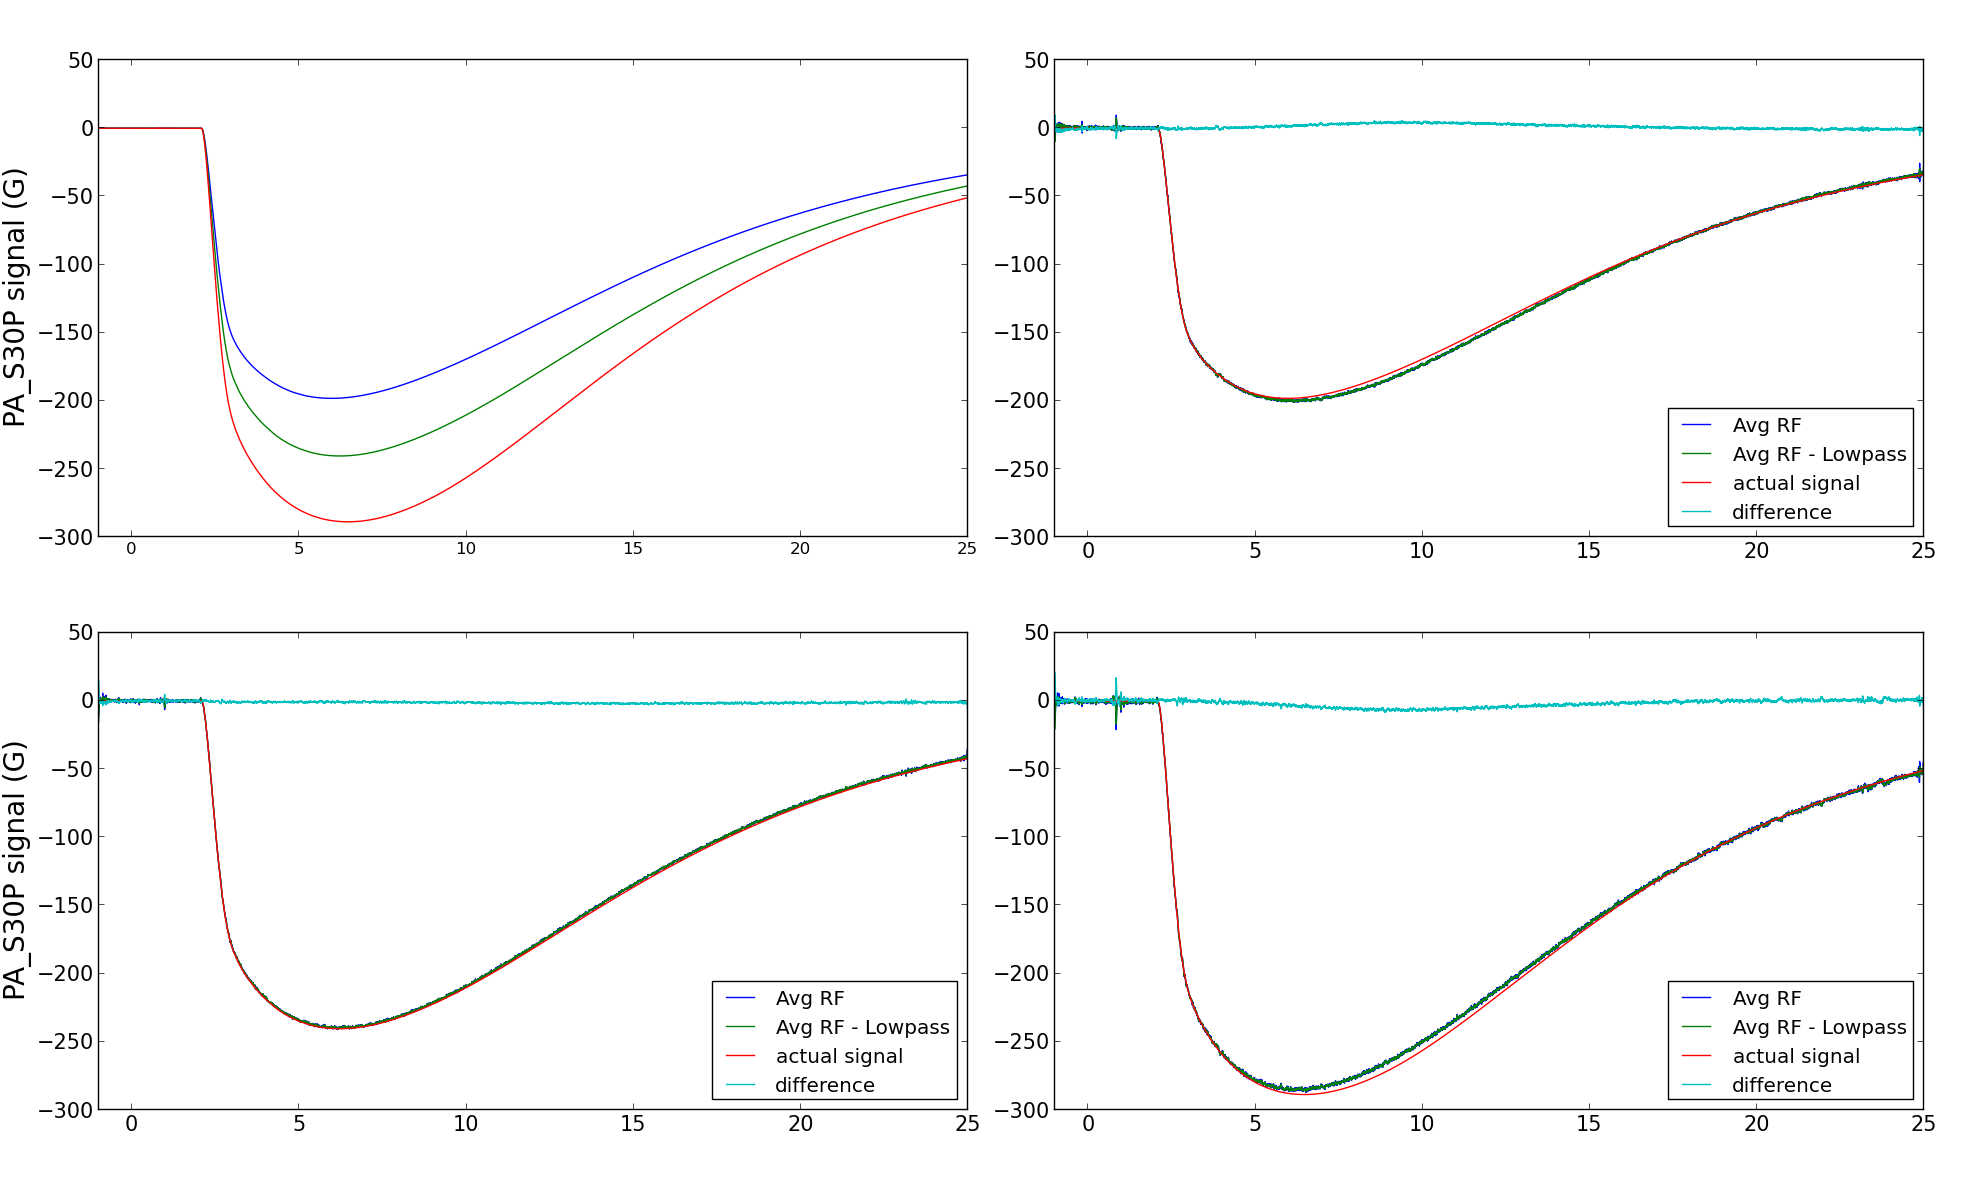
\includegraphics[width = \textwidth]{./sh_only_vac_subtract.png}\caption{Clockwise from top left: The three test cases of PA pickup of the shaping coil to be subtracted.  Each of the three cases, with the response function prediction overlaid, and the remainder after subtraction}
\label{raw_sig}
\end{figure}
\begin{center}
\begin{LARGE}
Subtracting pickup - Full vacuum field shots
\end{LARGE}
\end{center}
\par
The presence of additional vacuum fields are, however seen to affect the subtraction.  These effects vary from sensor to sensor, and between the same sensor on different poloidal arrays.  A variety of explanations present themselves, but which, or how many, are correct is an open question.
\par
We repeat the previous procedure.  A set of vacuum shots with all vacuum banks firing are taken, and a set of all banks save for the shaping coil, and the expected pickup based on the shaping current projected using the response function.  The vacuum shots had as similar a (non-shaping) vacuum field as possible across the data set.  With good subtraction, we should see measurements of the shaped vacuum fields (solid lines in the plots below) similar to that of shots without shaping fields (dashed lines).
\par 
We first looking at sensor PA\_S13P (or roughly 180$^{\circ}$ poloidally from the shaping coil) on both PA arrays.  OH \textbf{current} is in green, VF \textbf{current} is in magenta, and shaping \textbf{current} is in red.  PA \textbf{field}, scaled for ease of comparison is in black.  The post-subtraction field is in yellow.  We see that indeed, the response function for this sensor is essentially zero.  That is, the dashed and solid black lines are equivalent, showing no pickup, and the yellow lines are the same, showing no predicted effect of the shaping current.
\begin{figure}[h!]
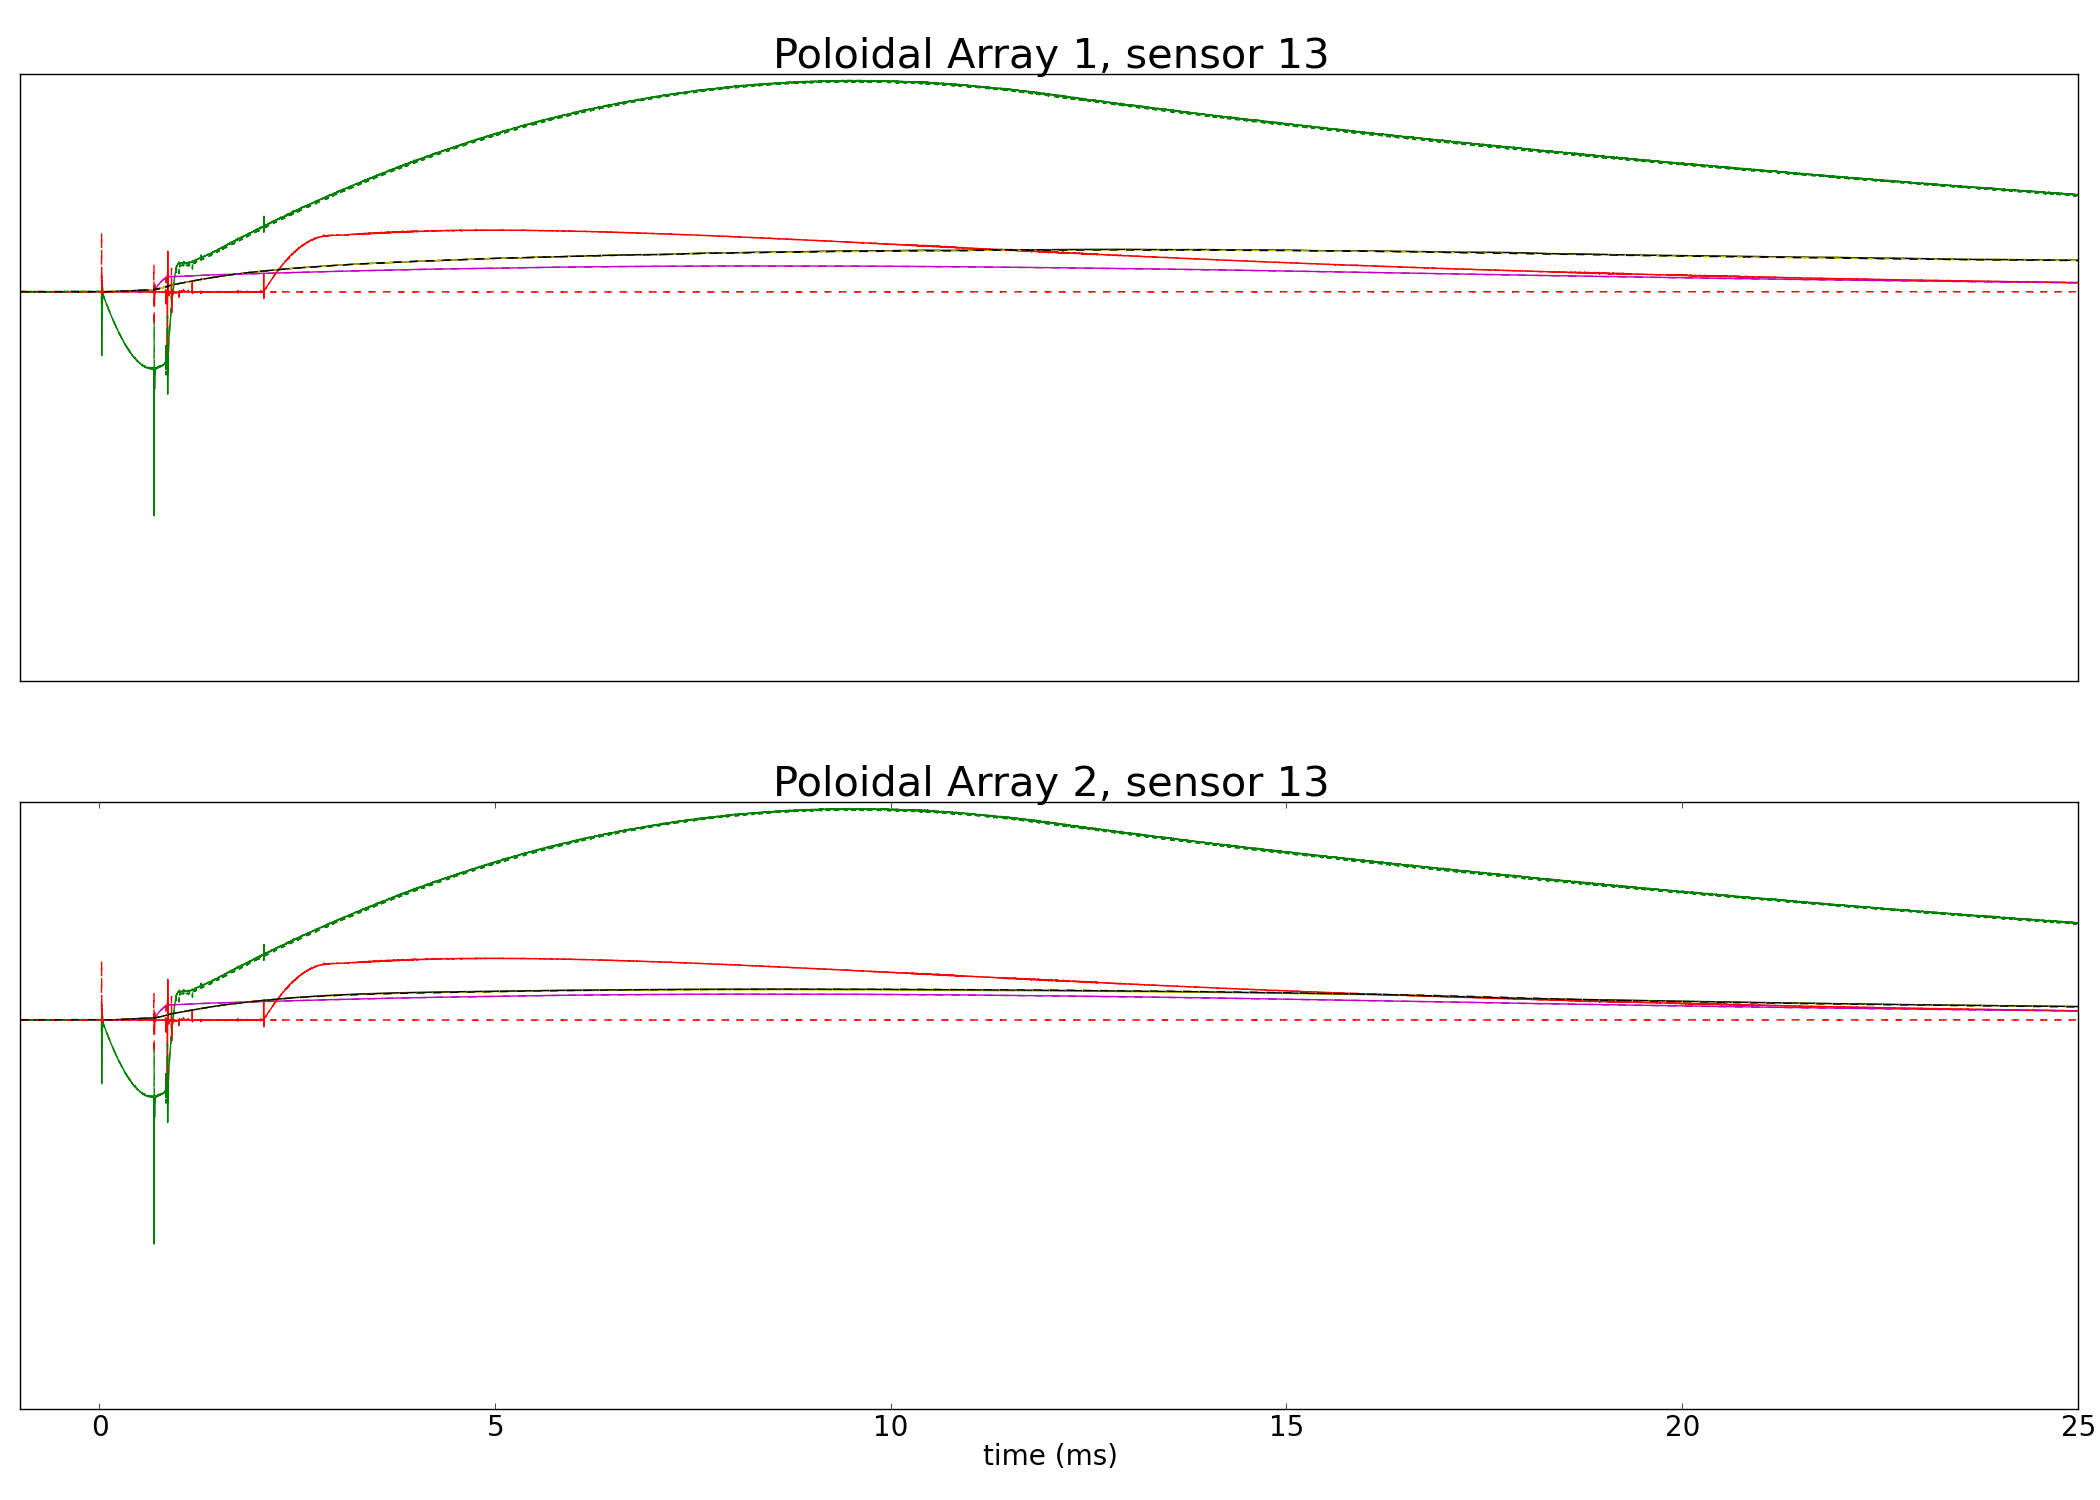
\includegraphics[width = \textwidth]{./RF_subtraction_results_vacuum_sensor_13.png}\caption{Subtraction in sensor 13.  The Shaping coil is not seen to influence the pickup, and the Response function subtraction has minimal influence, as expected.}
\label{raw_sig}
\end{figure}
\par
Once we begin to look at more complicated fields the subtraction becomes poorer.  For example, PA\_S30P has rather good subtraction in PA1, but there is a significant over-subtraction in PA2.  Why the field should be lower than expected in the presence of the other coils' field is as yet unresolved.
\begin{figure}[h!]
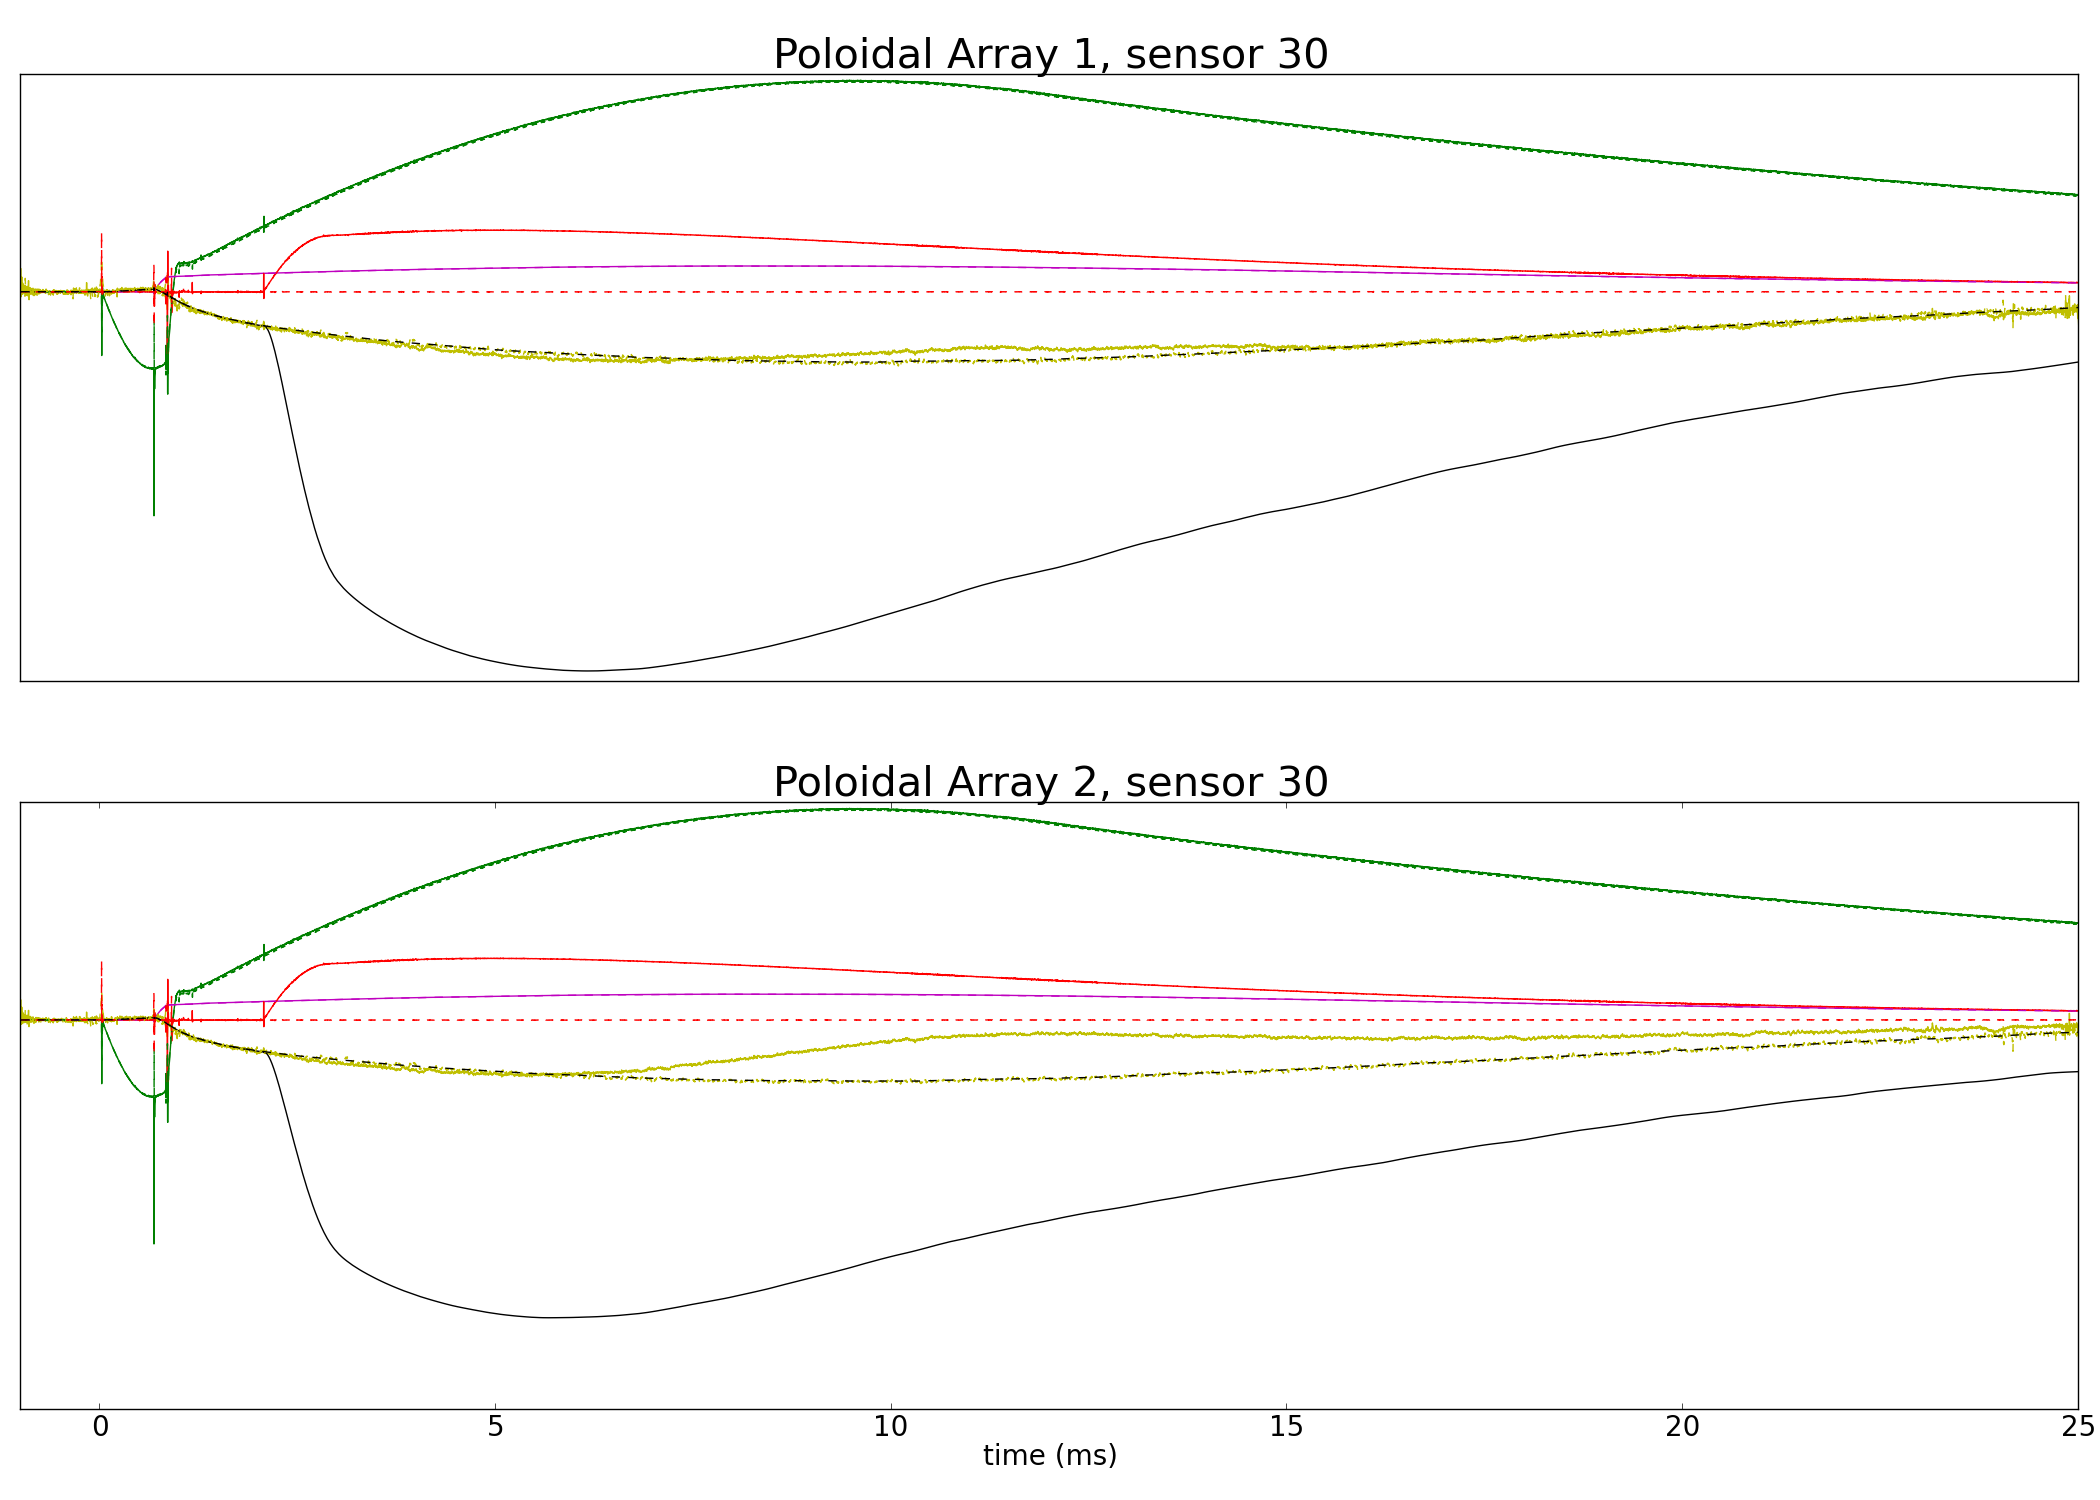
\includegraphics[width = \textwidth]{./RF_subtraction_results_vacuum_sensor_30.png}\caption{Subtraction in sensor 30.  Good preformance in sensor 1, poor performance in sensor 2 after 6ms}
\label{raw_sig}
\end{figure}
\par
The situation is further complicated by looking at other sensors.  For instance, sensor 32, at the inboard midplane, has similar disagreements, but the sensors are transposed.  In this case, PA1 begins to have large disagreement after about 5ms, while PA2 seems to be quite good throughout the likely lifetime of a plasma.
\begin{figure}[h!]
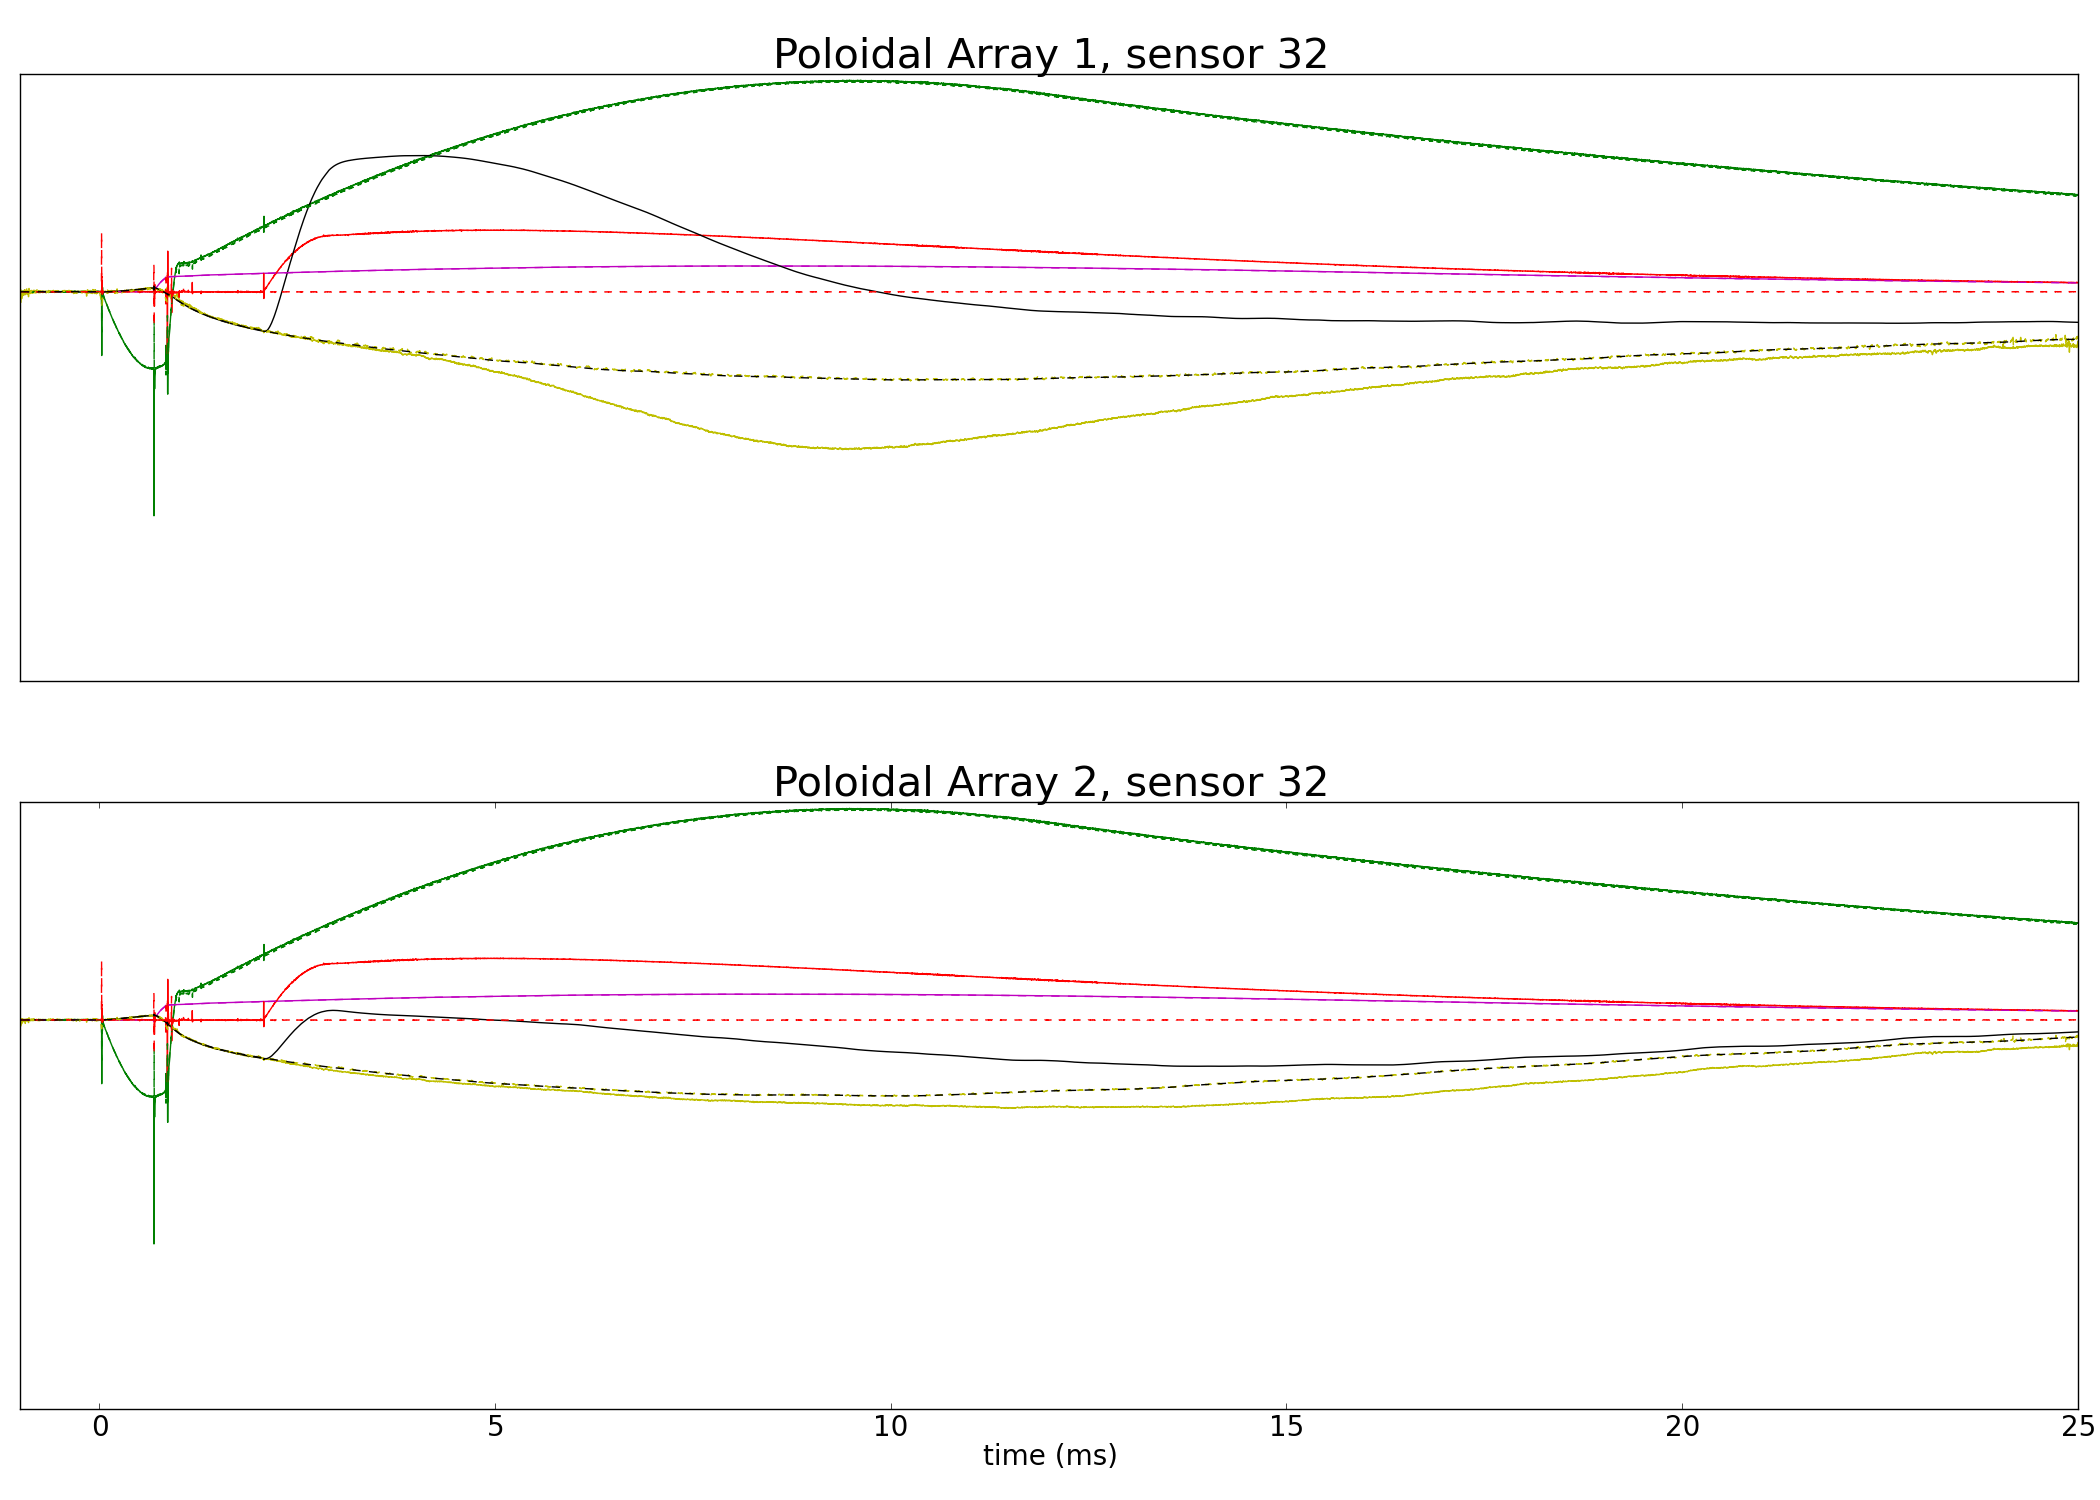
\includegraphics[width = \textwidth]{./RF_subtraction_results_vacuum_sensor_32.png}\caption{Subtraction in sensor 30.  Good preformance in sensor 1, poor performance in sensor 2 after 6ms}
\label{raw_sig}
\end{figure}
\end{document}